\newpage
\hypertarget{growBox vis}{}
\subsection{Implementing grow}
\visHeader

\begin{itemize}
 
\item[$\blacktriangleright$] Start by creating the simple story pattern depicted in Fig.~\ref{ea:sdm_growContext}. This matches the box and \emph{any} two
partitions.\footnote{Remember, the \emph{pattern matcher} is non-deterministic.}

\vspace{0.5cm}

\begin{figure}[htbp]
\begin{center}
  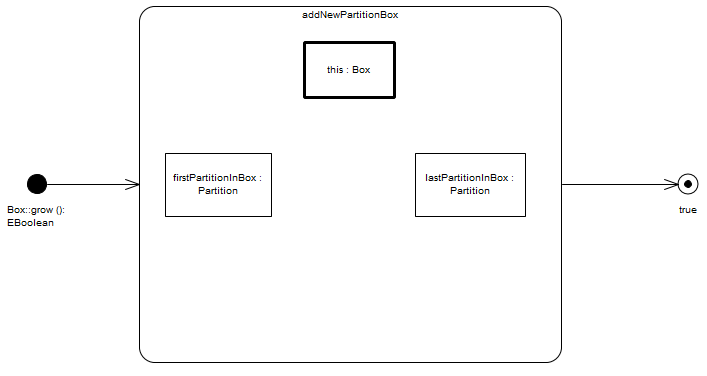
\includegraphics[width=\textwidth]{ea_elementsGrowBox}
  \caption{Context elements for SDM}  
  \label{ea:sdm_growContext}
\end{center}
\end{figure}

\item[$\blacktriangleright$] To create an appropriate \mbox{NAC} to constrain the possible matches for \texttt{lastPartitionInBox},  create a new
\texttt{Partition} object variable \texttt{next\-Part\-ition} and set its \emph{binding semantics} to \texttt{negative} (Fig.~\ref{ea:sdm_negOV}). The object
variable should now be visualised as being cancelled or struck out.
 
\begin{figure}[htbp]
\begin{center}
  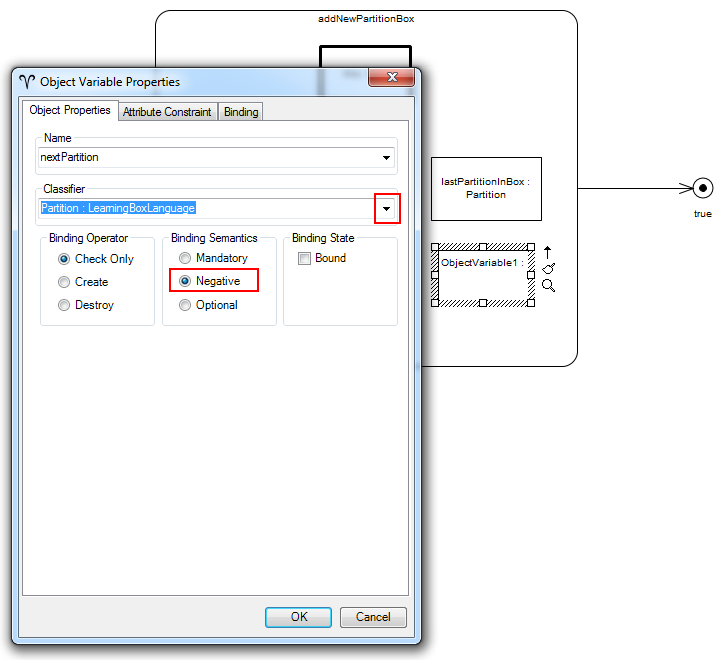
\includegraphics[width=0.7\textwidth]{ea_newNac}
  \caption{Adding a negative element}  
  \label{ea:sdm_negOV}
\end{center}
\end{figure}
 
\item[$\blacktriangleright$] Now, quick link \texttt{nextPartition} to \texttt{lastPartitionInBox}. Be sure to choose the link type carefully! The
\texttt{nextPartition} should play the role of \texttt{next} with respect to \texttt{lastPartitionInBox}. This combination (the negative binding and reference)
tells the pattern matcher that if the (assumed) last partition has an element connected via its \texttt{next} reference, the current match is invalid.

\item[$\blacktriangleright$] Great work -- the first NAC is complete! In a similar fashion, create the NAC for \texttt{firstPartitionInBox}. Name the
negative element \texttt{previousPartition}, and again, be sure to double-check the link variable.

\item[$\blacktriangleright$] Finally, complete the pattern so that it closely resembles Fig.~\ref{ea:sdm_firstLastPartitions}. 

\begin{figure}[htbp]
\begin{center}
  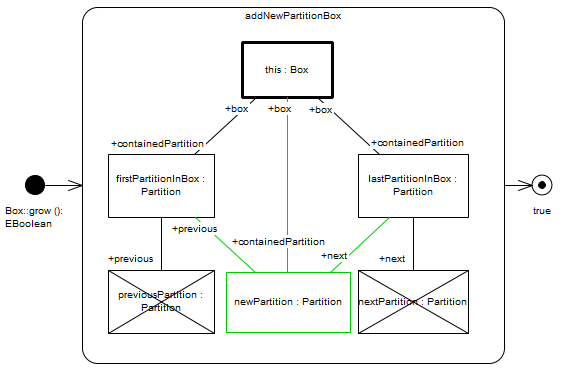
\includegraphics[width=\textwidth]{ea_NACComplete} 
  \caption{Determining the first and last partitions with NACs}  
  \label{ea:sdm_firstLastPartitions}
\end{center}
\end{figure}
 
\item[$\blacktriangleright$] Notice how the created partition \texttt{newPartition} is `hung' into the box. It becomes the next partition of the current
\emph{last} partition, and its previous partition is automatically set to the first partition in the box (as dictated by the rules set in
Fig.~\ref{fig:membox_depiction}). In other words, the new partition is appended onto the current set of partitions.

\item[$\blacktriangleright$] In order to complete \texttt{grow}, we need to set the size of the \texttt{newPartition}. Given that the new size is calculated
via the helper function \texttt{det\-er\-mine\-Next\-Size}, we need to use a \emph{MethodCallExpression}. Go ahead and invoke the corresponding dialogue,
activate the assignment (\texttt{:=}) operator, and match your values to Fig.~\ref{ea:sdm_methodCallExpr}.
 
\begin{figure}[htbp]
\begin{center}
  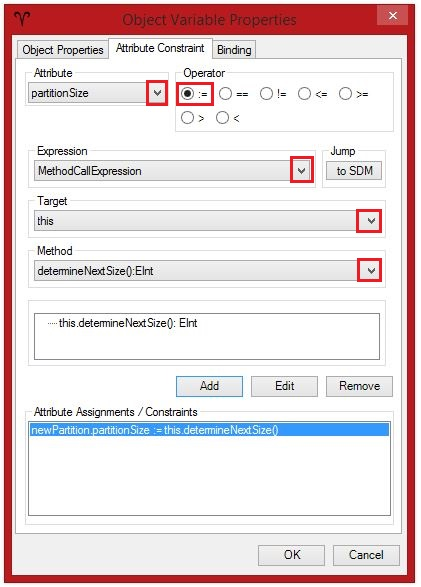
\includegraphics[width=0.6\textwidth]{ea_attributeMethodCall}
  \caption{Invoking a method via a \texttt{MethodCallExpression}}  
  \label{ea:sdm_methodCallExpr} 
\end{center}
\end{figure}

\item[$\blacktriangleright$] Since \texttt{determineNextSize} doesn't require any parameters, you can ignore the \texttt{Parameter Values} field this time. 

\vspace{0.5cm}

\item[$\blacktriangleright$] If you've done everything right, your SDM should now closely resemble Fig.~\ref{ea:growComplete}. As usual, try to export,
generate code, and inspect the method implementation in Eclipse.

\vspace{0.5cm}

\item[$\blacktriangleright$]  That's it -- the \texttt{grow} SDM is complete! This was probably the most challenging SDM to build so give yourself a solid 
pat on the back. If you found it easy, well then \ldots I guess I'm doing my job correctly. To see how this is done in the texual syntax, review
Fig.~\ref{eclipse:patternComplete}.

\vspace{0.5cm}

\begin{figure}[htbp]
\begin{center}
  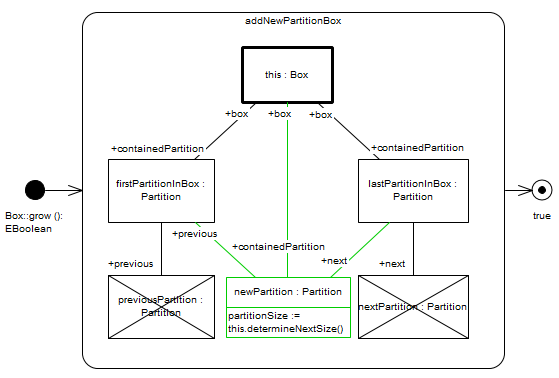
\includegraphics[width=\textwidth]{ea_growFinal}
  \caption{Complete SDM for \texttt{Box::grow}}  
  \label{ea:growComplete}
\end{center}
\end{figure}
\FloatBarrier

\jumpSingle{sec:conBran}

\end{itemize}
